\documentclass{pset}

\renewcommand{\hmwkTitle}{3rd\ hw}
\renewcommand{\hmwkDueDate}{February 12, 2014}
\renewcommand{\hmwkClass}{Algebraic Topology}
\renewcommand{\hmwkClassTime}{Section 1.2}
\renewcommand{\hmwkAuthorName}{}


\begin{document}

\maketitle

\pagebreak 

\begin{problem}
    \begin{enumerate}[label=1.2.\arabic*]
        \setcounter{enumi}{6}
        \item We can endow $X$ with a cell structure by letting $X^0$ be a singleton and $X^1$ be homeo $S^1 \vee S^1$ by attaching two 1-cells in the obvious way, and then we can obtain $X$ by attaching \textbf{two} 2-cells through a map that takes the upper semicircle of the boundary of the 2-cell to the first circle in $S^1 \vee S^1$ and the lower semicircle to the second. (see diagram below.) Now we can apply proposition 1.26.a to see that
        \[\pi_1(X) \cong \pi_1(S^1 \vee S^1)/N \cong <a, b>/N \cong <a, ab>/N\]
        such that $N$ is the normal group generated by the loops that the characteristic maps of the 2-cells generate. But both generate the same loop that goes through both circles in $S^1 \vee S^1$ once. Therefore,
        \[\pi_1(X) \cong \bZ\]
        
        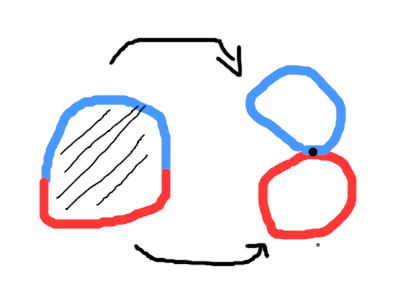
\includegraphics[width=4cm]{cell attachment.png}
        \setcounter{enumi}{8}
        \item 

        \setcounter{enumi}{16}
        \item 
        \item \begin{enumerate}[label=(\alph*)]
            \item Let the quotient map of $SX$ be $q$ and put $A_i = q\bigl(\{0, 1/i\} \times I \cup \{1/n \mid n \neq i\} \times ([0, .25) \cup (.75, 1]\bigr)$ which are evidently open, and each deformation retracts to $S^1$, and they satisfy the assumptions of Van Kampen. Furthermore, $A_i \cap A_j$ for all $i \neq j$ is contractible. Hence,
            \[\pi_1(SX) = \bigast^\i \bZ\]
        \end{enumerate}
    \end{enumerate}
\end{problem}
\begin{problem}
    \begin{enumerate}
        \item Let $\bR^*$ be the line with two origins and $0$ and $0'$ are the two origins. Suppose $f$ is a loop and let $F\colon I \times I \to \bR^*$ be a homotopy between $f$ and a loop that never traverses $0'$ defined as
        \[F(s, t) = 
        \begin{cases}
            f(s) & f(s) \neq 0' \\
            0' & f(s) = 0', t<1/2 \\
            0 & f(s) = 0', t\geq 1/2
        \end{cases}\]
        note that $F^{-1}(\{0, 0'\}) = f^{-1}(\{0, 0'\}) \times I$ and $F^{-1}(S) = f^{-1}(S) \times I$ for any set $S \subset \bR^*$ such that $S \cap \{0, 0'\} = \varnothing$. Now let $O$ be an open subset of $\bR^*$. $O$ either contains both $0$ and $0'$ or neither; if it didn't, $F^{-1}(O)$ is obviously open and if it did
        \[F^{-1}(O) = F^{-1}(\{0, 0'\}) \cup F^{-1}(O \setminus \{0, 0'\}) = f^{-1}(\{0, 0'\}) \times I \cup f^{-1}(O \setminus \{0, 0'\}) \times I = f^{-1}(O) \times I\]
        which is open hence $F$ is continuous
    \end{enumerate}
\end{problem}
\end{document}
